% !TEX program = xelatex
% AI-effects 프로젝트 --- 산업 집단의 AI 사용(점유율 지표 A·B·C)과 노출도 비교.
% 표 본문: results/table/39_main.tex, 39_abc.tex, 39_decomp.tex, 39_top.tex
%          (code/04_23_analysis_kor_industry_usage.do가 생성; 집단 자료는 code/01_09_import_kostat_regional_groups.do)
% 설명 대상: results/table/39_kor_industry_usage.xlsx, results/figure/39_fig_ind_{R,decomp}.{png,pdf}
% 관련: paper 38(같은 방법의 성별·연령·교육·임금 집단), 27(지표), 33(척도와 부트스트랩)
% 컴파일: xelatex -> biber -> xelatex -> xelatex (kotex, biblatex/biber 필요)
\documentclass[11pt]{article}

\usepackage{fontspec}
\usepackage{kotex}
\usepackage[a4paper,margin=2.0cm]{geometry}
\usepackage{longtable}
\usepackage{booktabs}
\usepackage{array}
\usepackage{amsmath}
\usepackage{xcolor}
\usepackage{hyperref}
\usepackage{enumitem}
\usepackage{graphicx}
\usepackage[backend=biber,style=authoryear,maxcitenames=2,uniquelist=false,sorting=nyt]{biblatex}
\addbibresource{../../reference/references.bib}

\hypersetup{colorlinks=true,linkcolor=blue!50!black,urlcolor=blue!50!black}
\newcolumntype{L}[1]{>{\raggedright\arraybackslash}p{#1}}
\newcolumntype{R}[1]{>{\raggedleft\arraybackslash}p{#1}}
\setlength{\LTleft}{0pt}
\setlength{\LTright}{0pt}
\renewcommand{\arraystretch}{1.15}
\setlength{\tabcolsep}{3.5pt}

\title{산업별 AI 사용과 노출도\\[2mm]
\large --- KSIC 11차 대분류와 국민계정 제조업 13개 산업 ---}
\author{AI-effects 프로젝트}
\date{\today}

\begin{document}
\maketitle

\begin{abstract}
\noindent paper 38의 집단 분석을 산업으로 넓혔다. 직업(KSCO 8차 소분류) 단위의 AI 사용 점유율 지표 A$\cdot$B$\cdot$C(paper 27)와 노출도 3개(Felten AIOE\parencite{felten-2023-how-will-language-modelers-like-chatgpt}, Eloundou $\beta$\parencite{eloundou-2023-gpts-are-gpts-an-early}, Observed Exposure\parencite{massenkoff-2026-labor-market-impacts-of-ai})를 지역별고용조사 2022년 상반기의 직업 $\times$ 산업 취업자 구성으로 산업에 나누었다. 산업분류는 두 가지다. (1) 한국표준산업분류(KSIC) 11차 대분류 21개, (2) 제조업 밖은 KSIC 대분류, 제조업은 국민계정 13개 산업(C01$\sim$C13)인 33개다. AEI는 사용자의 산업을 공개하지 않으므로, 같은 직업 안에서는 산업과 관계없이 1인당 사용이 같다고 가정한다. 산업 차이는 모두 직업 구성의 차이다.
\begin{itemize}[leftmargin=*]
  \item \textbf{사용은 정보통신과 전문 서비스에 몰려 있다.} 취업자 가중 평균을 1로 둔 사용 강도 $R$(지표 C)은 J 정보통신업 7.58, M 전문$\cdot$과학$\cdot$기술 서비스업 3.66, R 예술$\cdot$스포츠$\cdot$여가 3.01, K 금융$\cdot$보험업 2.26이다. 정보통신업은 취업자의 3.5\%인데 사용의 26.5\%를 가진다.
  \item \textbf{사용이 적은 산업}: A 농림어업(0.03), I 숙박$\cdot$음식점업(0.05), H 운수$\cdot$창고업(0.16), B 광업(0.17), F 건설업(0.30), Q 보건$\cdot$사회복지(0.32), G 도소매업(0.43). 제조업은 0.60이다.
  \item \textbf{노출도에 비해서도 차이가 크다.} 노출도의 산업 차이는 사용보다 훨씬 작다(Eloundou $\beta$ 0.46$\sim$2.00). 사용이 노출도의 몇 배인지를 나타내는 로그 거리는 J $+1.33$, M $+0.77$이고, I $-2.43$, H $-1.82$, L 부동산업 $-1.06$, G $-1.05$다. 도소매$\cdot$부동산은 노출도가 평균보다 높은데 사용은 평균의 절반 아래다.
  \item \textbf{제조업 안에서는 차이가 작다.} 국민계정 13개 산업의 사용 강도는 0.25(C01 음식료품)$\sim$1.05(C05 화학물질 및 화학제품)이고, C05와 C09 컴퓨터$\cdot$전자$\cdot$광학기기(0.90)를 빼면 모두 0.75 아래다. 노출도도 0.73$\sim$1.15로 좁다.
  \item \textbf{차이는 대부분 전문가 직업의 비중에서 나온다.} 정보통신업의 사용 몫이 취업자 몫보다 23.0\%p 큰데 그중 22.3\%p가 전문가 대분류다. 제조업의 몫이 6.4\%p 작은 것은 주로 장치$\cdot$기계 조작($-5.4$\%p) 직업 때문이다.
\end{itemize}
\end{abstract}

\section{산업분류와 방법}

\begin{itemize}[leftmargin=*]
  \item \textbf{자료}: 지역별고용조사 2022년 상반기 취업자의 \texttt{3자리\_11차산업소분류코드}(KSIC 11차 소분류). 코드 앞 두 자리(중분류)로 대분류를 정했다(A 01$\sim$03, B 05$\sim$08, C 10$\sim$34, D 35, E 36$\sim$39, F 41$\sim$42, G 45$\sim$47, H 49$\sim$52, I 55$\sim$56, J 58$\sim$63, K 64$\sim$66, L 68, M 70$\sim$73, N 74$\sim$76, O 84, P 85, Q 86$\sim$87, R 90$\sim$91, S 94$\sim$96, T 97$\sim$98, U 99). 취업자 모두 코드가 있다.
  \item \textbf{분류 (1)}: KSIC 11차 대분류 21개.
  \item \textbf{분류 (2)}: 제조업 밖은 KSIC 대분류 20개, 제조업은 국민계정 13개 산업. 대응은 한국은행 『우리나라의 국민계정체계(2025)』 <표 Ⅲ-2-6>$\cdot$<표 Ⅲ-2-7>의 KSIC 코드를 중분류로 묶은 것이다: C01 음식료품 10$\sim$12, C02 섬유 및 가죽제품 13$\sim$15, C03 목재$\cdot$종이$\cdot$인쇄 및 복제 16$\sim$18, C04 코크스 및 석유정제품 19, C05 화학물질 및 화학제품 20$\sim$22(의약품, 고무$\cdot$플라스틱 포함), C06 비금속광물제품 23, C07 1차금속 24, C08 금속가공제품 25, C09 컴퓨터$\cdot$전자 및 광학기기 26$\sim$27, C10 전기장비 28, C11 기계 및 장비 29, C12 운송장비 30$\sim$31, C13 기타 제조업 및 산업용 장비 수리 32$\sim$34.
  \item 두 분류에서 제조업 밖 20개 산업의 값은 같다(do 파일에서 확인). 그래서 표는 분류 (1)의 21개와 분류 (2)의 제조업 13개만 싣는다. 분류 (2) 전체는 엑셀에 있다.
  \item \textbf{방법}: paper 38과 같다. 소분류 점유율을 산업 취업자(B는 근로시간) 구성비로 나눠 합 1로 정규화하고, 사용 강도 $R$ = 산업 몫 / 취업자(근로시간) 비중, 상대 노출도 $RX$ = 산업 취업자 가중 노출도 / 전체 평균, 로그 거리 $d = \ln R - \ln RX$를 구한다. 구간은 소분류 163개를 복원추출한 부트스트랩 999회의 95\% 백분위 구간이다. 대상은 취업자 전체이고, 사용 0인 34개 소분류는 사용 0으로 들어간다.
\end{itemize}

\section{결과}

\subsection{사용 강도와 노출도}

\begin{small}
\begin{longtable}{L{4.6cm}R{1.2cm}R{1.1cm}R{2.7cm}R{1.2cm}R{1.2cm}R{2.8cm}R{1.2cm}}
\caption{산업별 사용(지표 C)과 노출도. $R$ = 사용 강도, $RX$ = 상대 노출도, $d = \ln R - \ln RX$. 대괄호는 부트스트랩 95\% 구간}\label{tab:main}\\
\toprule
산업 & 취업자(\%) & C(\%) & $R$ & $RX$($\beta$) & $RX$(OE) & $d$($\beta$) & $d$(OE) \\
\midrule
\endfirsthead
\toprule
산업 & 취업자(\%) & C(\%) & $R$ & $RX$($\beta$) & $RX$(OE) & $d$($\beta$) & $d$(OE) \\
\midrule
\endhead
% 04_23_analysis_kor_industry_usage.do가 생성. 직접 고치지 말 것.
\multicolumn{8}{l}{\textit{KSIC 11차 대분류}} \\
\quad A 농업, 임업 및 어업 & 5.5 & 0.2 & 0.03 {\footnotesize [0.01, 0.59]} & 0.46 & 0.03 & -2.79 {\footnotesize [-4.54, -0.12]} & -0.09 \\
\quad B 광업 & 0.0 & 0.0 & 0.17 {\footnotesize [0.06, 0.43]} & 0.78 & 0.60 & -1.54 {\footnotesize [-2.36, -0.82]} & -1.29 \\
\quad C 제조업 & 16.1 & 9.7 & 0.60 {\footnotesize [0.40, 0.96]} & 0.91 & 0.71 & -0.41 {\footnotesize [-0.81, 0.04]} & -0.17 \\
\quad D 전기, 가스, 증기 및 공기 조절 공급업 & 0.3 & 0.3 & 1.17 {\footnotesize [0.59, 1.99]} & 1.31 & 1.14 & -0.12 {\footnotesize [-0.82, 0.44]} & +0.03 \\
\quad E 수도, 하수 및 폐기물 처리, 원료 재생업 & 0.6 & 0.4 & 0.64 {\footnotesize [0.25, 1.47]} & 1.00 & 0.69 & -0.45 {\footnotesize [-1.29, 0.33]} & -0.08 \\
\quad F 건설업 & 7.6 & 2.3 & 0.30 {\footnotesize [0.16, 0.61]} & 0.70 & 0.57 & -0.85 {\footnotesize [-1.36, -0.35]} & -0.65 \\
\quad G 도매 및 소매업 & 11.9 & 5.1 & 0.43 {\footnotesize [0.23, 1.05]} & 1.23 & 1.67 & -1.05 {\footnotesize [-1.56, -0.33]} & -1.35 \\
\quad H 운수 및 창고업 & 5.9 & 1.0 & 0.16 {\footnotesize [0.07, 0.56]} & 1.01 & 0.53 & -1.82 {\footnotesize [-2.62, -0.75]} & -1.18 \\
\quad I 숙박 및 음식점업 & 7.5 & 0.4 & 0.05 {\footnotesize [0.02, 0.16]} & 0.54 & 0.25 & -2.43 {\footnotesize [-3.41, -1.30]} & -1.65 \\
\quad J 정보통신업 & 3.5 & 26.5 & 7.58 {\footnotesize [4.49, 11.98]} & 2.00 & 3.31 & +1.33 {\footnotesize [0.92, 1.84]} & +0.83 \\
\quad K 금융 및 보험업 & 2.5 & 5.7 & 2.26 {\footnotesize [0.96, 6.48]} & 1.51 & 2.22 & +0.40 {\footnotesize [-0.29, 1.35]} & +0.02 \\
\quad L 부동산업 & 1.9 & 0.9 & 0.47 {\footnotesize [0.15, 1.03]} & 1.34 & 1.82 & -1.06 {\footnotesize [-2.04, -0.20]} & -1.36 \\
\quad M 전문, 과학 및 기술 서비스업 & 4.5 & 16.4 & 3.66 {\footnotesize [2.39, 5.85]} & 1.69 & 1.70 & +0.77 {\footnotesize [0.40, 1.21]} & +0.77 \\
\quad N 사업시설 관리, 사업 지원 및 임대 서비스업 & 5.2 & 3.7 & 0.71 {\footnotesize [0.38, 1.36]} & 0.91 & 0.99 & -0.25 {\footnotesize [-0.79, 0.27]} & -0.33 \\
\quad O 공공 행정, 국방 및 사회보장 행정 & 4.6 & 7.3 & 1.59 {\footnotesize [0.60, 4.30]} & 1.07 & 0.75 & +0.40 {\footnotesize [-0.50, 1.39]} & +0.75 \\
\quad P 교육 서비스업 & 6.8 & 10.1 & 1.49 {\footnotesize [0.77, 2.96]} & 1.15 & 1.55 & +0.26 {\footnotesize [-0.33, 0.91]} & -0.04 \\
\quad Q 보건업 및 사회복지 서비스업 & 9.7 & 3.1 & 0.32 {\footnotesize [0.19, 0.57]} & 0.84 & 0.62 & -0.97 {\footnotesize [-1.51, -0.42]} & -0.67 \\
\quad R 예술, 스포츠 및 여가관련 서비스업 & 1.7 & 5.2 & 3.01 {\footnotesize [0.98, 6.45]} & 1.09 & 1.15 & +1.02 {\footnotesize [-0.02, 1.65]} & +0.96 \\
\quad S 협회 및 단체, 수리 및 기타 개인 서비스업 & 3.9 & 1.8 & 0.46 {\footnotesize [0.24, 0.97]} & 0.83 & 0.76 & -0.60 {\footnotesize [-1.11, 0.01]} & -0.51 \\
\quad T 가구 내 고용활동 및 자가 소비 생산활동 & 0.3 & 0.1 & 0.45 {\footnotesize [0.04, 0.70]} & 0.54 & 0.26 & -0.17 {\footnotesize [-2.48, 0.23]} & +0.57 \\
\quad U 국제 및 외국기관 & 0.0 & 0.0 & 0.38 {\footnotesize [0.08, 1.04]} & 0.96 & 0.78 & -0.94 {\footnotesize [-2.36, 0.21]} & -0.73 \\
\midrule
\multicolumn{8}{l}{\textit{제조업 세부: 국민계정 13개 산업}} \\
\quad C01 음식료품 & 1.6 & 0.4 & 0.25 {\footnotesize [0.11, 0.62]} & 0.79 & 0.50 & -1.14 {\footnotesize [-1.80, -0.40]} & -0.69 \\
\quad C02 섬유 및 가죽제품 & 1.2 & 0.5 & 0.43 {\footnotesize [0.15, 1.24]} & 0.79 & 0.62 & -0.60 {\footnotesize [-1.61, 0.20]} & -0.36 \\
\quad C03 목재, 종이, 인쇄 및 복제 & 0.7 & 0.4 & 0.59 {\footnotesize [0.22, 1.55]} & 0.97 & 0.73 & -0.49 {\footnotesize [-1.47, 0.34]} & -0.21 \\
\quad C04 코크스 및 석유정제품 & 0.1 & 0.0 & 0.48 {\footnotesize [0.13, 1.50]} & 0.98 & 0.74 & -0.70 {\footnotesize [-1.80, 0.15]} & -0.42 \\
\quad C05 화학물질 및 화학제품 & 2.0 & 2.1 & 1.05 {\footnotesize [0.31, 2.99]} & 0.99 & 0.75 & +0.06 {\footnotesize [-1.09, 0.97]} & +0.34 \\
\quad C06 비금속광물제품 & 0.4 & 0.2 & 0.44 {\footnotesize [0.19, 0.98]} & 0.90 & 0.82 & -0.72 {\footnotesize [-1.40, -0.01]} & -0.62 \\
\quad C07 1차금속 & 0.6 & 0.2 & 0.38 {\footnotesize [0.13, 1.10]} & 0.79 & 0.50 & -0.74 {\footnotesize [-1.65, 0.12]} & -0.29 \\
\quad C08 금속가공제품 & 1.4 & 0.5 & 0.35 {\footnotesize [0.15, 0.79]} & 0.78 & 0.61 & -0.81 {\footnotesize [-1.55, -0.09]} & -0.57 \\
\quad C09 컴퓨터, 전자 및 광학기기 & 2.3 & 2.1 & 0.90 {\footnotesize [0.49, 1.69]} & 1.15 & 0.92 & -0.24 {\footnotesize [-0.69, 0.25]} & -0.02 \\
\quad C10 전기장비 & 1.0 & 0.5 & 0.55 {\footnotesize [0.28, 1.12]} & 1.02 & 0.81 & -0.61 {\footnotesize [-1.18, -0.03]} & -0.39 \\
\quad C11 기계 및 장비 & 1.8 & 1.2 & 0.63 {\footnotesize [0.30, 1.24]} & 1.00 & 0.84 & -0.45 {\footnotesize [-1.12, 0.15]} & -0.28 \\
\quad C12 운송장비 & 2.1 & 0.9 & 0.42 {\footnotesize [0.13, 1.17]} & 0.73 & 0.59 & -0.55 {\footnotesize [-1.50, 0.16]} & -0.33 \\
\quad C13 기타 제조업 및 산업용 장비 수리 & 0.9 & 0.6 & 0.72 {\footnotesize [0.30, 1.47]} & 0.86 & 0.72 & -0.19 {\footnotesize [-1.11, 0.52]} & -0.00 \\

\bottomrule
\end{longtable}
\end{small}

\begin{figure}[htbp]
\centering
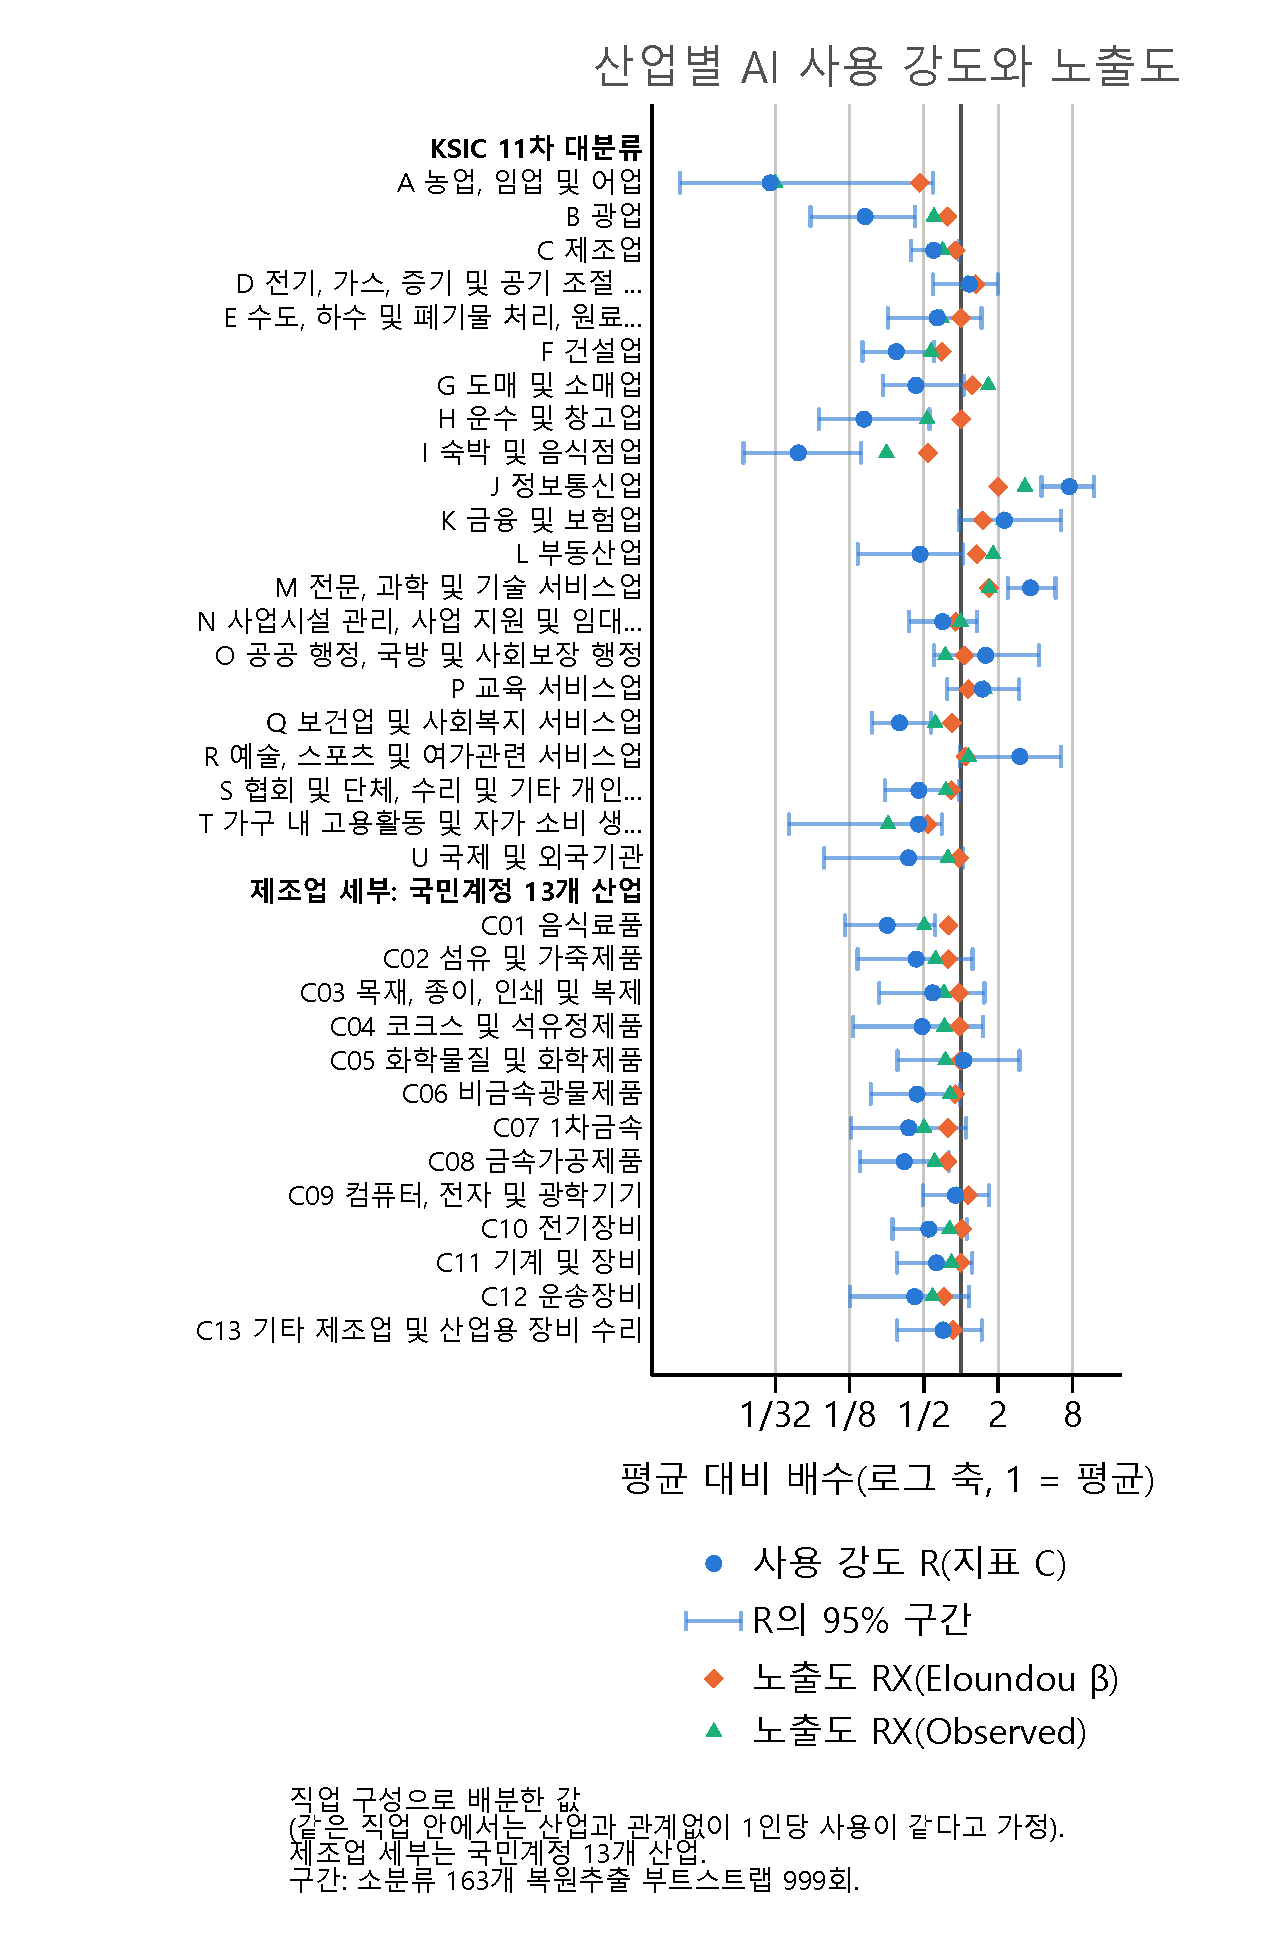
\includegraphics[width=0.72\textwidth]{../figure/39_fig_ind_R.pdf}
\caption{산업별 사용 강도 $R$(지표 C, 95\% 구간)과 상대 노출도 $RX$(Eloundou $\beta$, Observed). 로그 축, 1 = 취업자 전체 평균}\label{fig:R}
\end{figure}

\paragraph{사용이 많은 산업.} J 정보통신업의 사용 강도는 7.58 [4.49, 11.98]로 평균의 7배를 넘는다. 노출도도 가장 높지만($\beta$ 2.00, OE 3.31) 사용이 그보다 훨씬 크다($d$ = $+1.33$). M 전문$\cdot$과학$\cdot$기술 서비스업(3.66)과 R 예술$\cdot$스포츠$\cdot$여가(3.01)가 뒤를 잇는다. K 금융$\cdot$보험업(2.26), O 공공행정(1.59), P 교육(1.49)도 평균보다 높지만 구간이 넓다. 예를 들어 K의 구간은 [0.96, 6.48]이다. 이 산업들의 사용이 소수 직업(표~\ref{tab:top})에 기대고 있어, 그 직업이 표본에 드느냐에 따라 값이 크게 움직이기 때문으로 보인다.

\paragraph{사용이 적은 산업.} A 농림어업(0.03), I 숙박$\cdot$음식점업(0.05), H 운수$\cdot$창고업(0.16), B 광업(0.17), F 건설업(0.30), Q 보건$\cdot$사회복지(0.32)는 평균의 3분의 1에도 못 미친다. 노출도는 이보다 덜 낮아서 로그 거리가 크게 음수다(I $-2.43$, A $-2.79$, H $-1.82$). G 도소매업(사용 0.43, 노출도 1.23$\cdot$1.67)과 L 부동산업(0.47, 1.34$\cdot$1.82)은 노출도가 평균보다 높은데 사용은 평균의 절반 아래다. 판매$\cdot$중개 직업이 많아 노출도는 높게 잡히지만 실제 업무용 대화는 적다는 직업 단위 결과(paper 28$\cdot$29)가 산업에서도 나타난다.

\paragraph{제조업.} 제조업 전체의 사용 강도는 0.60 [0.40, 0.96], 노출도는 0.91($\beta$)$\cdot$0.71(OE)이다. 국민계정 13개 산업으로 나누면 C05 화학물질 및 화학제품(1.05)과 C09 컴퓨터$\cdot$전자 및 광학기기(0.90)가 가장 높고, C01 음식료품(0.25), C08 금속가공제품(0.35), C07 1차금속(0.38)이 가장 낮다. 노출도의 폭(0.73$\sim$1.15)이 좁아 제조업 안의 차이는 산업 간 차이에 비해 작다. 구간이 대부분 겹치므로 제조업 세부 순위는 조심해서 읽어야 한다.

\subsection{지표 A$\cdot$B$\cdot$C와 배분 방식}

\begin{small}
\begin{longtable}{L{4.6cm}R{1.6cm}R{1.3cm}R{1.3cm}R{2.2cm}R{1.3cm}R{3.2cm}}
\caption{근로시간 비중, 지표별 사용 강도, Felten AIOE 평균의 차이(산업 평균 $-$ 전체 평균, 대괄호는 95\% 구간)}\label{tab:abc}\\
\toprule
산업 & 근로시간(\%) & $R^{\mathrm{A}}$ & $R^{\mathrm{B}}$ & $R^{\mathrm{B}}$(취업자 배분) & $R^{\mathrm{C}}$ & Felten 차이 \\
\midrule
\endfirsthead
\toprule
산업 & 근로시간(\%) & $R^{\mathrm{A}}$ & $R^{\mathrm{B}}$ & $R^{\mathrm{B}}$(취업자 배분) & $R^{\mathrm{C}}$ & Felten 차이 \\
\midrule
\endhead
% 04_23_analysis_kor_industry_usage.do가 생성. 직접 고치지 말 것.
\multicolumn{7}{l}{\textit{KSIC 11차 대분류}} \\
\quad A 농업, 임업 및 어업 & 5.0 & 0.03 & 0.03 & 0.03 & 0.03 & -0.83 {\footnotesize [-1.04, -0.56]} \\
\quad B 광업 & 0.1 & 0.17 & 0.16 & 0.17 & 0.17 & -0.51 {\footnotesize [-0.83, 0.09]} \\
\quad C 제조업 & 17.3 & 0.58 & 0.59 & 0.63 & 0.60 & -0.31 {\footnotesize [-0.54, -0.06]} \\
\quad D 전기, 가스, 증기 및 공기 조절 공급업 & 0.3 & 1.22 & 1.17 & 1.23 & 1.17 & +0.26 {\footnotesize [-0.09, 0.59]} \\
\quad E 수도, 하수 및 폐기물 처리, 원료 재생업 & 0.6 & 0.58 & 0.64 & 0.66 & 0.64 & -0.24 {\footnotesize [-0.49, 0.15]} \\
\quad F 건설업 & 7.8 & 0.32 & 0.31 & 0.31 & 0.30 & -0.58 {\footnotesize [-0.89, -0.11]} \\
\quad G 도매 및 소매업 & 12.6 & 0.50 & 0.42 & 0.44 & 0.43 & +0.44 {\footnotesize [0.21, 0.87]} \\
\quad H 운수 및 창고업 & 6.5 & 0.19 & 0.15 & 0.17 & 0.16 & -0.35 {\footnotesize [-0.57, 0.24]} \\
\quad I 숙박 및 음식점업 & 7.8 & 0.07 & 0.05 & 0.05 & 0.05 & -0.38 {\footnotesize [-0.61, -0.10]} \\
\quad J 정보통신업 & 3.6 & 7.60 & 7.64 & 7.72 & 7.58 & +0.75 {\footnotesize [0.47, 0.97]} \\
\quad K 금융 및 보험업 & 2.6 & 2.52 & 2.35 & 2.36 & 2.26 & +0.92 {\footnotesize [0.63, 1.22]} \\
\quad L 부동산업 & 2.0 & 0.50 & 0.48 & 0.48 & 0.47 & +0.38 {\footnotesize [-0.31, 0.92]} \\
\quad M 전문, 과학 및 기술 서비스업 & 4.6 & 3.35 & 3.58 & 3.71 & 3.66 & +0.72 {\footnotesize [0.53, 0.91]} \\
\quad N 사업시설 관리, 사업 지원 및 임대 서비스업 & 5.3 & 0.85 & 0.68 & 0.71 & 0.71 & -0.25 {\footnotesize [-0.51, 0.14]} \\
\quad O 공공 행정, 국방 및 사회보장 행정 & 4.1 & 1.38 & 1.71 & 1.55 & 1.59 & -0.04 {\footnotesize [-0.45, 0.37]} \\
\quad P 교육 서비스업 & 5.8 & 1.28 & 1.47 & 1.32 & 1.49 & +0.77 {\footnotesize [0.37, 0.99]} \\
\quad Q 보건업 및 사회복지 서비스업 & 8.1 & 0.39 & 0.36 & 0.31 & 0.32 & +0.08 {\footnotesize [-0.18, 0.36]} \\
\quad R 예술, 스포츠 및 여가관련 서비스업 & 1.6 & 3.31 & 2.93 & 2.93 & 3.01 & +0.19 {\footnotesize [-0.01, 0.43]} \\
\quad S 협회 및 단체, 수리 및 기타 개인 서비스업 & 4.1 & 0.50 & 0.44 & 0.45 & 0.46 & -0.00 {\footnotesize [-0.37, 0.47]} \\
\quad T 가구 내 고용활동 및 자가 소비 생산활동 & 0.2 & 0.28 & 0.45 & 0.32 & 0.45 & -0.18 {\footnotesize [-0.53, 0.03]} \\
\quad U 국제 및 외국기관 & 0.0 & 0.43 & 0.15 & 0.38 & 0.38 & -0.09 {\footnotesize [-0.52, 0.20]} \\
\midrule
\multicolumn{7}{l}{\textit{제조업 세부: 국민계정 13개 산업}} \\
\quad C01 음식료품 & 1.7 & 0.24 & 0.25 & 0.27 & 0.25 & -0.38 {\footnotesize [-0.64, 0.05]} \\
\quad C02 섬유 및 가죽제품 & 1.3 & 0.48 & 0.43 & 0.45 & 0.43 & -0.46 {\footnotesize [-0.72, 0.17]} \\
\quad C03 목재, 종이, 인쇄 및 복제 & 0.7 & 0.57 & 0.55 & 0.58 & 0.59 & -0.34 {\footnotesize [-0.67, 0.25]} \\
\quad C04 코크스 및 석유정제품 & 0.1 & 0.45 & 0.48 & 0.50 & 0.48 & -0.20 {\footnotesize [-0.58, 0.48]} \\
\quad C05 화학물질 및 화학제품 & 2.1 & 0.88 & 1.05 & 1.09 & 1.05 & -0.24 {\footnotesize [-0.57, 0.33]} \\
\quad C06 비금속광물제품 & 0.5 & 0.43 & 0.42 & 0.45 & 0.44 & -0.29 {\footnotesize [-0.65, 0.17]} \\
\quad C07 1차금속 & 0.6 & 0.34 & 0.37 & 0.40 & 0.38 & -0.50 {\footnotesize [-0.86, 0.07]} \\
\quad C08 금속가공제품 & 1.5 & 0.36 & 0.34 & 0.36 & 0.35 & -0.48 {\footnotesize [-0.78, 0.01]} \\
\quad C09 컴퓨터, 전자 및 광학기기 & 2.5 & 0.92 & 0.90 & 0.95 & 0.90 & -0.04 {\footnotesize [-0.39, 0.37]} \\
\quad C10 전기장비 & 1.1 & 0.53 & 0.53 & 0.58 & 0.55 & -0.15 {\footnotesize [-0.45, 0.24]} \\
\quad C11 기계 및 장비 & 2.0 & 0.62 & 0.63 & 0.67 & 0.63 & -0.21 {\footnotesize [-0.53, 0.19]} \\
\quad C12 운송장비 & 2.3 & 0.43 & 0.42 & 0.45 & 0.42 & -0.46 {\footnotesize [-0.77, 0.01]} \\
\quad C13 기타 제조업 및 산업용 장비 수리 & 0.9 & 0.71 & 0.68 & 0.74 & 0.72 & -0.39 {\footnotesize [-0.65, -0.02]} \\

\bottomrule
\end{longtable}
\end{small}

지표와 배분 방식을 바꿔도 사용 강도의 순서는 거의 같다. 차이가 가장 큰 곳은 O 공공행정($R^{\mathrm{A}}$ 1.38, $R^{\mathrm{B}}$ 1.71)과 R 예술$\cdot$스포츠$\cdot$여가(3.31, 2.93)처럼 대화당 절감 시간이 평균과 다른 직업이 많은 산업이다. Felten AIOE로 보면 K 금융$\cdot$보험($+0.92$), P 교육($+0.77$), J 정보통신($+0.75$), M 전문서비스($+0.72$)가 높고, A 농림어업($-0.83$), F 건설($-0.58$)이 낮다. P 교육은 Felten 차이가 큰 데 비해 Eloundou 노출도는 1.15로 평균에 가깝다.

\subsection{차이는 어느 직업에서 오는가}

\begin{small}
\begin{longtable}{L{4.0cm}R{1.3cm}R{1.3cm}R{1.3cm}R{1.3cm}R{1.3cm}R{1.3cm}R{1.3cm}R{1.3cm}}
\caption{산업 몫 $-$ 취업자 몫(\%p)의 직업 대분류별 기여: 사용(지표 C)과 노출도(Eloundou $\beta$ 기반 점유율)}\label{tab:decomp}\\
\toprule
 & \multicolumn{2}{c}{C 제조업} & \multicolumn{2}{c}{J 정보통신} & \multicolumn{2}{c}{M 전문$\cdot$과학$\cdot$기술} & \multicolumn{2}{c}{Q 보건$\cdot$사회복지} \\
직업 대분류 & 사용 & 노출도 & 사용 & 노출도 & 사용 & 노출도 & 사용 & 노출도 \\
\midrule
\endfirsthead
% 04_23_analysis_kor_industry_usage.do가 생성. 직접 고치지 말 것.
1 관리자 & +1.1 & +0.1 & +0.7 & +0.0 & +0.7 & +0.0 & +0.2 & +0.0 \\
2 전문가 및 관련 종사자 & +4.6 & +1.2 & +22.3 & +2.7 & +10.9 & +1.5 & -3.0 & +0.1 \\
3 사무 종사자 & -2.7 & +3.3 & +0.3 & +0.8 & +0.5 & +1.6 & +0.1 & +0.6 \\
4 서비스 종사자 & -0.1 & -0.0 & -0.0 & -0.0 & -0.0 & -0.0 & -2.2 & -1.1 \\
5 판매 종사자 & -0.3 & -0.0 & -0.1 & +0.0 & -0.0 & -0.0 & -0.0 & +0.0 \\
6 농림∙어업 숙련 종사자 & -0.0 & -0.0 & 0.0 & 0.0 & -0.0 & -0.0 & -0.0 & -0.0 \\
7 기능원 및 관련 기능 종사자 & -2.2 & -1.5 & -0.1 & -0.0 & -0.1 & -0.0 & +0.0 & -0.0 \\
8 장치∙기계 조작 및 조립 종사자 & -5.4 & -3.7 & -0.0 & -0.0 & -0.0 & -0.0 & -0.1 & -0.0 \\
9 단순노무 종사자 & -1.5 & -0.8 & -0.1 & -0.0 & -0.0 & -0.0 & -1.6 & -1.1 \\
\midrule
합계(산업 몫 $-$ 취업자 몫) & -6.4 & -1.5 & +23.0 & +3.5 & +11.9 & +3.1 & -6.6 & -1.5 \\

\bottomrule
\end{longtable}
\end{small}

\begin{figure}[htbp]
\centering
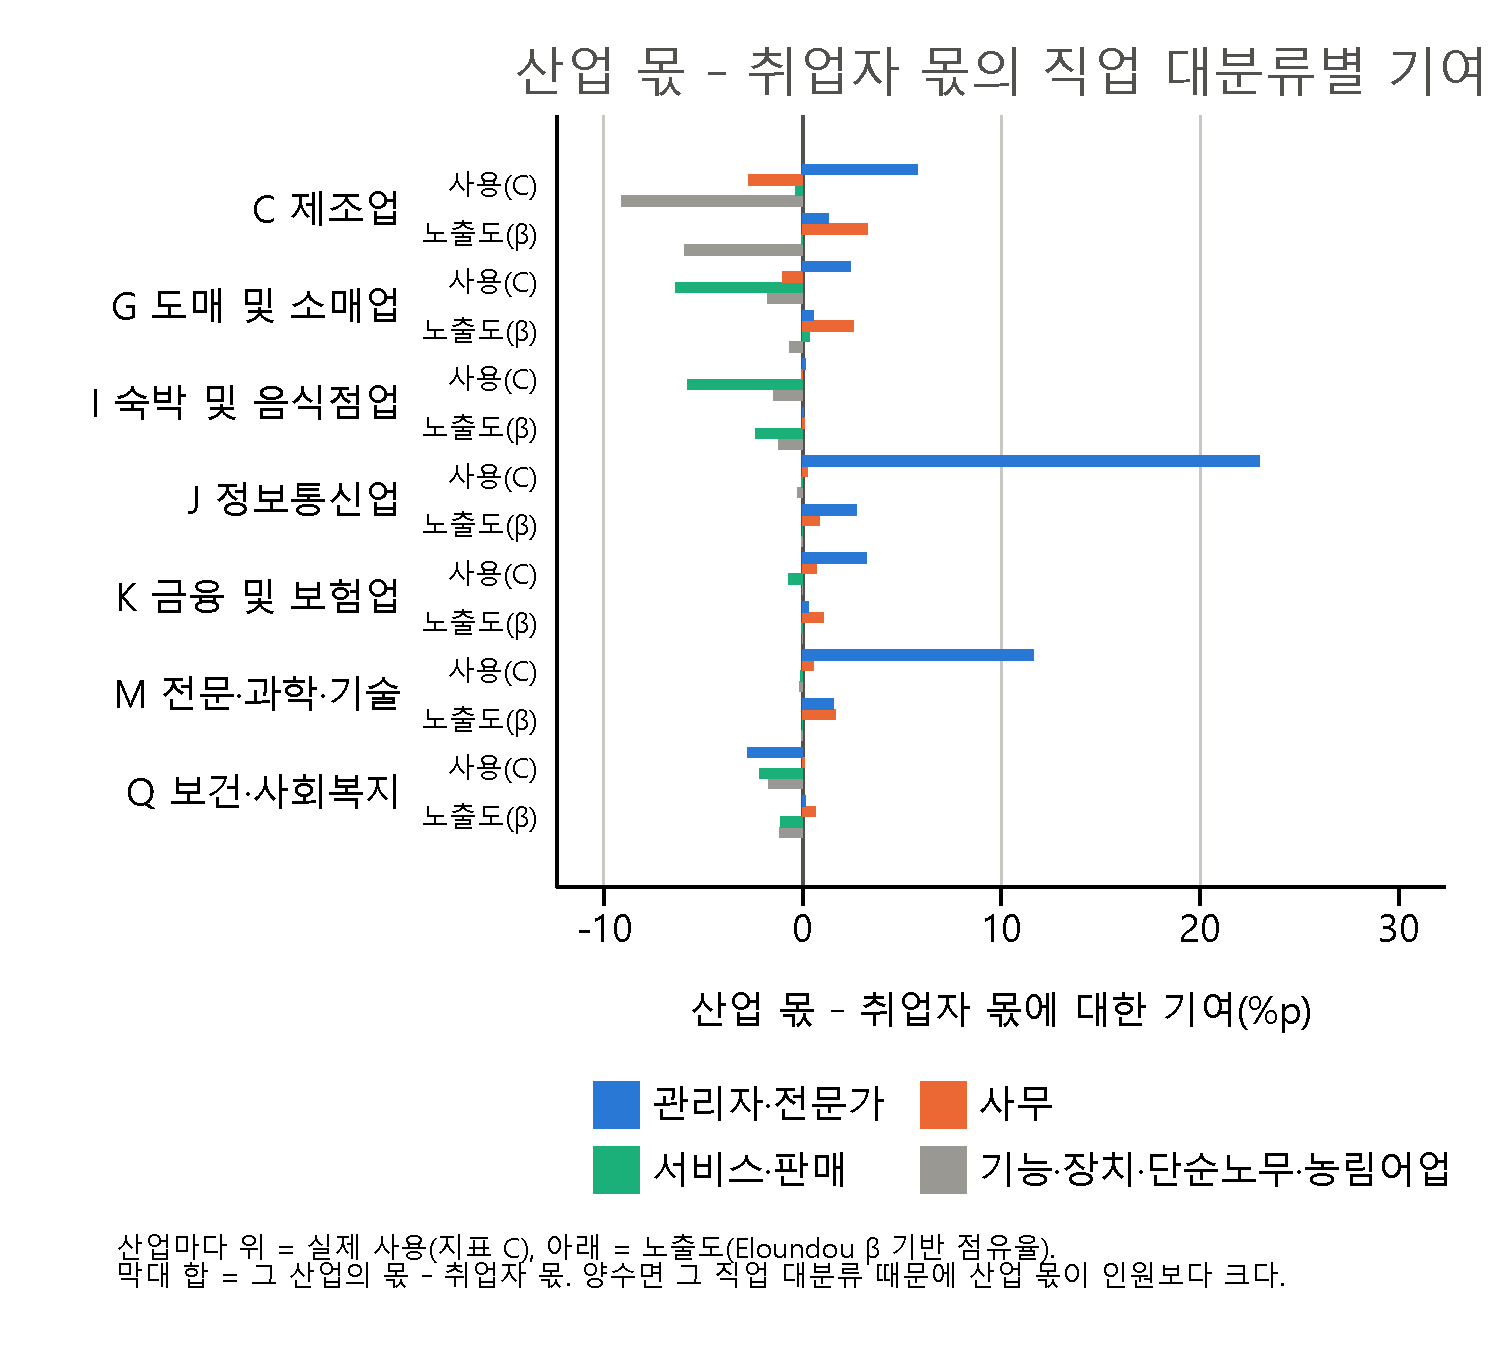
\includegraphics[width=0.85\textwidth]{../figure/39_fig_ind_decomp.pdf}
\caption{산업 몫 $-$ 취업자 몫의 직업 대분류별 기여(대분류 4묶음). 산업마다 위는 사용, 아래는 노출도}\label{fig:decomp}
\end{figure}

\begin{itemize}[leftmargin=*]
  \item \textbf{J 정보통신업}: 사용 몫이 취업자 몫보다 23.0\%p 크고, 그중 22.3\%p가 전문가 대분류(컴퓨터 시스템$\cdot$소프트웨어 전문가, 작가$\cdot$언론 등)다. 노출도 기준으로는 3.5\%p 클 뿐이다.
  \item \textbf{M 전문$\cdot$과학$\cdot$기술 서비스업}: 사용 몫이 11.9\%p 크고 거의 모두(10.9\%p) 전문가다. 노출도 기준은 3.1\%p다.
  \item \textbf{C 제조업}: 사용 몫이 6.4\%p 작다. 전문가(엔지니어$\cdot$시험원)가 $+4.6$\%p를 더하지만 장치$\cdot$기계 조작($-5.4$), 사무($-2.7$), 기능원($-2.2$), 단순노무($-1.5$)가 더 많이 뺀다. 노출도 기준으로는 $-1.5$\%p이고 사무가 $+3.3$\%p를 더한다.
  \item \textbf{Q 보건$\cdot$사회복지}: 사용 몫이 6.6\%p 작다. 전문가 대분류도 $-3.0$\%p다. 간호사 등 보건 전문직의 사용이 적기 때문이다(paper 29$\cdot$33). 서비스($-2.2$)와 단순노무($-1.6$)가 나머지를 뺀다.
\end{itemize}

\subsection{산업 안 사용의 분포}

\begin{footnotesize}
\begin{longtable}{L{3.0cm}L{4.2cm}L{4.2cm}L{4.2cm}R{1.2cm}}
\caption{산업 사용(지표 C) 중 몫이 큰 소분류 상위 3(괄호 = 산업 안 몫, \%)과 산업 안 실효 직업 수(1/HHI)}\label{tab:top}\\
\toprule
산업 & 1위 & 2위 & 3위 & 실효 직업 수 \\
\midrule
\endfirsthead
\toprule
산업 & 1위 & 2위 & 3위 & 실효 직업 수 \\
\midrule
\endhead
% 04_23_analysis_kor_industry_usage.do가 생성. 직접 고치지 말 것.
\multicolumn{5}{l}{\textit{KSIC 11차 대분류}} \\
\quad A 농업, 임업 및 어업 & 213 생명 및 자연과학 관련 시험원 (48.7) & 332 통계‧데이터 관련 사무원 (9.7) & 149 기타 건설‧전기 및 생산 관련 관리자 (9.4) & 3.7 \\
\quad B 광업 & 141 건설‧전기 및 생산 관련 관리자 (25.4) & 372 비서 및 사무 지원 종사자 (14.6) & 239 기타 공학 전문가 및 관련 종사자 (13.7) & 7.6 \\
\quad C 제조업 & 213 생명 및 자연과학 관련 시험원 (10.6) & 235 기계‧로봇공학 기술자 및 시험원 (9.2) & 222 컴퓨터 시스템 및 소프트웨어 전문가 (7.5) & 20.7 \\
\quad D 전기, 가스, 증기 및 공기 조절 공급업 & 861 발전 및 배전 장치 조작원 (31.0) & 852 냉난방 관련 설비 조작원 (10.7) & 236 소방‧방재‧산업안전 기술자 및 시험원 (9.4) & 7.3 \\
\quad E 수도, 하수 및 폐기물 처리, 원료 재생업 & 153 환경‧청소 및 경비 관련 관리자 (24.7) & 149 기타 건설‧전기 및 생산 관련 관리자 (21.9) & 237 환경공학‧가스‧에너지 기술자 및 시험원 (12.8) & 7.0 \\
\quad F 건설업 & 141 건설‧전기 및 생산 관련 관리자 (18.5) & 236 소방‧방재‧산업안전 기술자 및 시험원 (9.1) & 372 비서 및 사무 지원 종사자 (6.8) & 14.7 \\
\quad G 도매 및 소매업 & 283 상품 기획‧홍보 및 조사 전문가 (18.9) & 372 비서 및 사무 지원 종사자 (16.7) & 225 정보 시스템 및 웹 운영자 (6.5) & 11.5 \\
\quad H 운수 및 창고업 & 225 정보 시스템 및 웹 운영자 (23.2) & 372 비서 및 사무 지원 종사자 (15.1) & 151 판매 및 운송 관리자 (9.2) & 9.9 \\
\quad I 숙박 및 음식점업 & 152 고객 서비스 관리자 (28.7) & 283 상품 기획‧홍보 및 조사 전문가 (11.8) & 122 마케팅 및 광고‧홍보 관리자 (11.5) & 7.5 \\
\quad J 정보통신업 & 222 컴퓨터 시스템 및 소프트웨어 전문가 (36.7) & 291 작가 및 언론 관련 전문가 (22.3) & 225 정보 시스템 및 웹 운영자 (10.0) & 4.8 \\
\quad K 금융 및 보험업 & 282 금융 및 보험 전문가 (36.4) & 340 금융 사무 종사자 (26.0) & 225 정보 시스템 및 웹 운영자 (8.3) & 4.6 \\
\quad L 부동산업 & 284 감정‧기술 영업 및 중개 관련 종사자 (34.2) & 139 기타 전문 서비스 관리자 (32.6) & 372 비서 및 사무 지원 종사자 (8.5) & 4.2 \\
\quad M 전문, 과학 및 기술 서비스업 & 291 작가 및 언론 관련 전문가 (12.7) & 283 상품 기획‧홍보 및 조사 전문가 (11.0) & 211 생명 및 자연과학 관련 전문가 (10.1) & 16.0 \\
\quad N 사업시설 관리, 사업 지원 및 임대 서비스업 & 283 상품 기획‧홍보 및 조사 전문가 (20.9) & 372 비서 및 사무 지원 종사자 (8.4) & 522 상품 대여 종사자 (8.1) & 12.7 \\
\quad O 공공 행정, 국방 및 사회보장 행정 & 332 통계‧데이터 관련 사무원 (31.2) & 372 비서 및 사무 지원 종사자 (15.8) & 213 생명 및 자연과학 관련 시험원 (12.5) & 6.6 \\
\quad P 교육 서비스업 & 264 문리‧기술 및 예능 강사 (25.6) & 269 기타 교육 전문가 (17.6) & 261 대학교수 및 강사 (12.8) & 7.3 \\
\quad Q 보건업 및 사회복지 서비스업 & 372 비서 및 사무 지원 종사자 (13.3) & 246 치료‧재활사 및 의료기사 (10.6) & 291 작가 및 언론 관련 전문가 (9.6) & 15.9 \\
\quad R 예술, 스포츠 및 여가관련 서비스업 & 291 작가 및 언론 관련 전문가 (34.0) & 292 학예사‧사서 및 기록물 관리사 (21.0) & 298 문화‧예술 관련 기획자 (14.6) & 5.1 \\
\quad S 협회 및 단체, 수리 및 기타 개인 서비스업 & 372 비서 및 사무 지원 종사자 (13.3) & 291 작가 및 언론 관련 전문가 (9.9) & 149 기타 건설‧전기 및 생산 관련 관리자 (7.5) & 18.9 \\
\quad T 가구 내 고용활동 및 자가 소비 생산활동 & 951 가사 및 육아 도우미 (96.7) & 264 문리‧기술 및 예능 강사 (2.2) & 421 교사 보조 및 아동 돌봄 종사자 (0.6) & 1.1 \\
\quad U 국제 및 외국기관 & 283 상품 기획‧홍보 및 조사 전문가 (61.9) & 352 정부 행정 사무 종사자 (17.5) & 371 총무 사무원 및 대학 행정조교 (9.4) & 2.4 \\
\midrule
\multicolumn{5}{l}{\textit{제조업 세부: 국민계정 13개 산업}} \\
\quad C01 음식료품 & 239 기타 공학 전문가 및 관련 종사자 (17.0) & 121 행정 및 경영 지원 관리자 (10.5) & 141 건설‧전기 및 생산 관련 관리자 (8.8) & 13.0 \\
\quad C02 섬유 및 가죽제품 & 283 상품 기획‧홍보 및 조사 전문가 (44.0) & 721 섬유 및 가죽 관련 기능 종사자 (14.4) & 295 디자이너 (13.8) & 4.2 \\
\quad C03 목재, 종이, 인쇄 및 복제 & 291 작가 및 언론 관련 전문가 (29.6) & 122 마케팅 및 광고‧홍보 관리자 (19.1) & 799 기타 기능 관련 종사자 (9.3) & 6.7 \\
\quad C04 코크스 및 석유정제품 & 271 법률 전문가 (29.2) & 121 행정 및 경영 지원 관리자 (16.6) & 372 비서 및 사무 지원 종사자 (14.6) & 6.0 \\
\quad C05 화학물질 및 화학제품 & 213 생명 및 자연과학 관련 시험원 (46.5) & 211 생명 및 자연과학 관련 전문가 (16.4) & 332 통계‧데이터 관련 사무원 (4.1) & 4.0 \\
\quad C06 비금속광물제품 & 233 금속‧재료공학 기술자 및 시험원 (21.9) & 121 행정 및 경영 지원 관리자 (10.4) & 141 건설‧전기 및 생산 관련 관리자 (9.7) & 10.4 \\
\quad C07 1차금속 & 233 금속‧재료공학 기술자 및 시험원 (31.5) & 121 행정 및 경영 지원 관리자 (11.6) & 141 건설‧전기 및 생산 관련 관리자 (6.1) & 7.3 \\
\quad C08 금속가공제품 & 239 기타 공학 전문가 및 관련 종사자 (20.9) & 235 기계‧로봇공학 기술자 및 시험원 (11.7) & 225 정보 시스템 및 웹 운영자 (11.4) & 11.0 \\
\quad C09 컴퓨터, 전자 및 광학기기 & 222 컴퓨터 시스템 및 소프트웨어 전문가 (19.9) & 234 전기‧전자공학 기술자 및 시험원 (14.7) & 221 컴퓨터 하드웨어 및 통신공학 전문가 (8.3) & 11.0 \\
\quad C10 전기장비 & 222 컴퓨터 시스템 및 소프트웨어 전문가 (12.5) & 122 마케팅 및 광고‧홍보 관리자 (12.0) & 234 전기‧전자공학 기술자 및 시험원 (11.7) & 14.4 \\
\quad C11 기계 및 장비 & 235 기계‧로봇공학 기술자 및 시험원 (20.3) & 239 기타 공학 전문가 및 관련 종사자 (18.4) & 222 컴퓨터 시스템 및 소프트웨어 전문가 (11.0) & 9.6 \\
\quad C12 운송장비 & 235 기계‧로봇공학 기술자 및 시험원 (44.6) & 222 컴퓨터 시스템 및 소프트웨어 전문가 (8.3) & 239 기타 공학 전문가 및 관련 종사자 (8.2) & 4.5 \\
\quad C13 기타 제조업 및 산업용 장비 수리 & 730 목재‧가구‧악기 및 간판 관련 기능 종사자 (32.6) & 149 기타 건설‧전기 및 생산 관련 관리자 (26.3) & 295 디자이너 (8.1) & 5.2 \\

\bottomrule
\end{longtable}
\end{footnotesize}

산업 안 사용은 소수 직업에 몰려 있는 경우가 많다. 정보통신업은 222 컴퓨터 시스템 및 소프트웨어 전문가(36.7\%)와 291 작가 및 언론 관련 전문가(22.3\%)가 60\%를 차지해 실효 직업 수가 4.8개다. 직업 연계의 영향이 그대로 보이는 산업도 있다. A 농림어업의 사용은 절반 가까이(48.7\%)가 213 생명 및 자연과학 관련 시험원이고, C05 화학물질 및 화학제품도 46.5\%가 이 직업이다. 213은 취업자가 1만 1천 명인데 데이터 과학자 등 SOC의 대화가 연계표로 많이 배분된 직업이다(paper 23$\cdot$26). 산업 값에 이런 직업 하나가 크게 작용하므로, 사용 강도가 높게 나온 소규모 산업은 상위 직업을 함께 확인해야 한다.

\section{해석상 주의}

\begin{enumerate}[leftmargin=*]
  \item \textbf{직업 구성만 반영한다.} 같은 직업이면 어느 산업에서 일하든 1인당 사용이 같다고 가정했다. 같은 직업이라도 정보통신업 종사자가 제조업 종사자보다 더 많이 쓴다면 실제 산업 차이는 이보다 크다. AEI는 사용자의 산업을 공개하지 않아 이 가정을 점검할 수 없다.
  \item \textbf{직업 지표의 한계를 물려받는다.} 소분류 점유율은 연계표 배분(paper 21)에 의존하고, 사용 0인 34개 소분류(장치$\cdot$기계 조작 직업이 많음)는 공개되지 않은 것일 수 있다. 이 소분류들이 제조업$\cdot$운수업 값을 낮추는 방향으로 작용할 수 있다.
  \item \textbf{작은 산업.} U 국제 및 외국기관(표본 69명), T 가구 내 고용(386명), B 광업(252명), D 전기$\cdot$가스(707명)는 표본이 작고 구간이 넓다. 이 구간은 소분류 구성에 대한 것이고 조사 표본오차는 들어 있지 않다.
  \item \textbf{국민계정 대응의 범위.} 제조업 13개 산업은 KSIC 중분류 단위로 대응했다(한국은행 표의 소분류 구분은 모두 중분류 안에서 같은 산업으로 묶인다). 국민계정 산업분류에는 KSIC 대분류 U(국제 및 외국기관)가 없지만, 이번 분류 (2)는 제조업 밖을 KSIC 대분류로 두기로 했으므로 U를 따로 남겼다.
  \item \textbf{시점.} 산업 구성은 2022년 상반기, 사용은 2026년 4$\cdot$5월이다.
\end{enumerate}

\section{산출 파일}

\begin{itemize}[leftmargin=*]
  \item 코드: \texttt{code/01\_09\_import\_kostat\_regional\_groups.do}(산업 집단 ind1$\cdot$ind2 추가), \texttt{code/04\_23\_analysis\_kor\_industry\_usage.do}(산업 지표, 부트스트랩, 분해, 표$\cdot$그림). 둘 다 \texttt{00\_master.do}에 포함.
  \item 가공 자료: \texttt{data/proc/macro/kostat\_lfs\_regional/kostat\_lfs\_regional\_ksco3\_groups.\{dta,csv\}}(dim = ind1, ind2).
  \item 엑셀: \texttt{results/table/39\_kor\_industry\_usage.xlsx}. 시트 \texttt{groups}(두 분류의 모든 산업과 구간), \texttt{decomp}(모든 산업의 직업 대분류 9개별 기여, OE 포함), \texttt{top}(산업마다 상위 5 소분류).
  \item 이 노트의 표: \texttt{results/table/39\_main.tex}, \texttt{39\_abc.tex}, \texttt{39\_decomp.tex}, \texttt{39\_top.tex}.
  \item 그림: \texttt{results/figure/39\_fig\_ind\_R.\{pdf,png\}}, \texttt{39\_fig\_ind\_decomp.\{pdf,png\}}.
\end{itemize}

\printbibliography[title={참고문헌}]

\end{document}
